\section{Error Consistency \& Human Alignment}
In \cref{subsec:error consistency}, we described results for testing ViT-22B fine-tuned on ImageNet on the \texttt{model-vs-human} benchmark. In \cref{fig:model_vs_human_benchmark_a}, \cref{fig:model_vs_human_benchmark_b}, \cref{fig:model_vs_human_benchmark_c}, \cref{fig:model_vs_human_benchmark_d}, we provide additional benchmarking results.

\begin{figure}[ht]
    \centering
    \subfigure[][OOD accuracy (higher = better).]{
        \label{fig:model_vs_human_benchmark_a}
        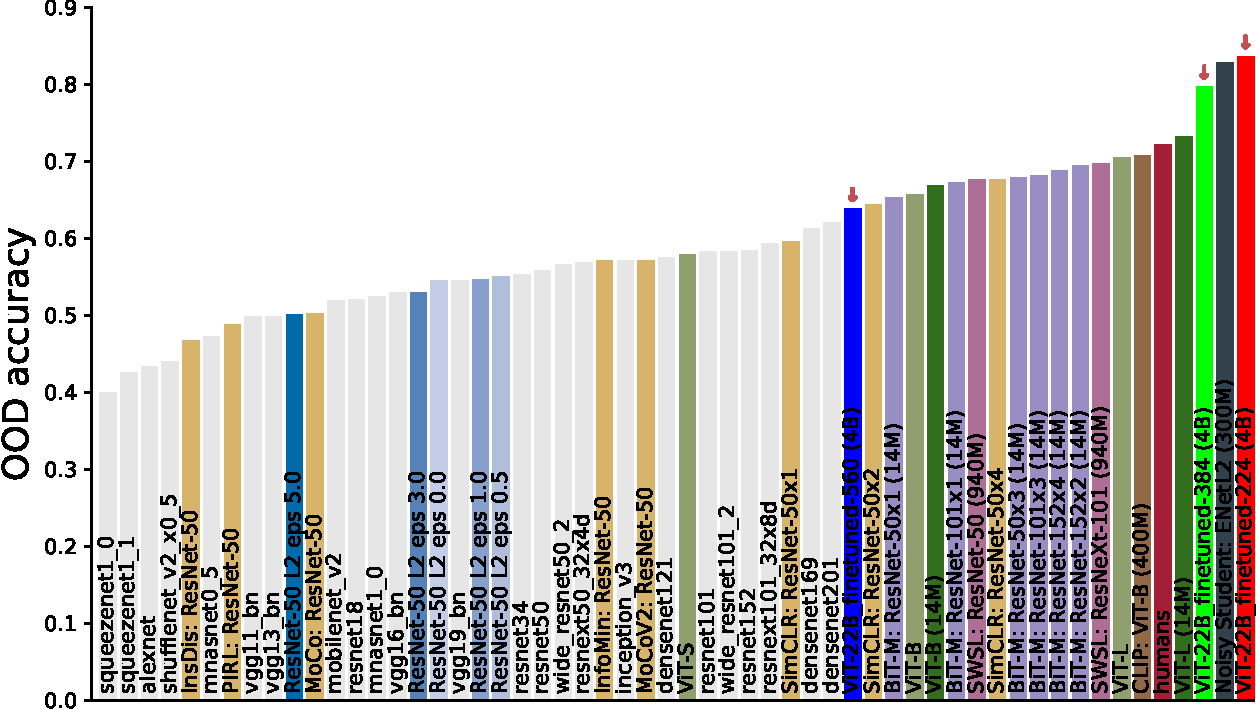
\includegraphics[height=1.6in]{figs/human-alignment/benchmark_16-class-accuracy.pdf}}
    \hspace{8pt}
    \subfigure[][Accuracy difference (lower = better).]{
        \label{fig:model_vs_human_benchmark_b}%
        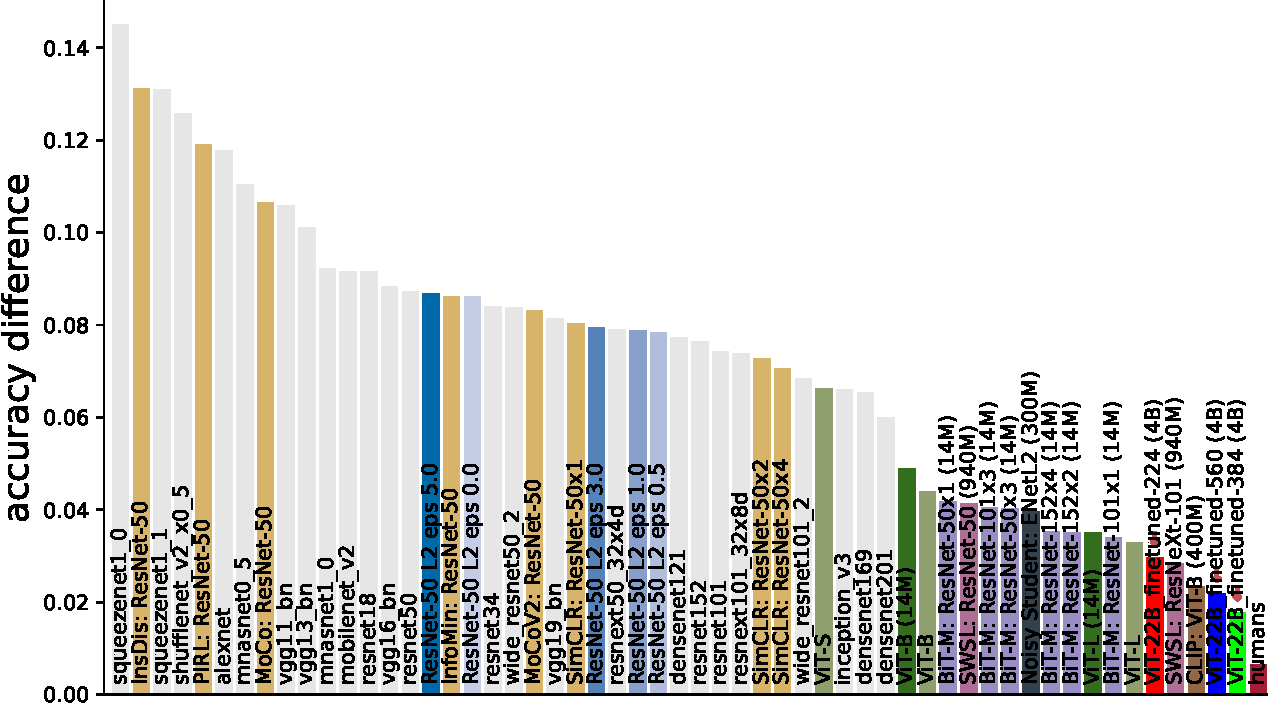
\includegraphics[height=1.6in]{figs/human-alignment/benchmark_16-class-accuracy-difference.pdf}} \\
    \subfigure[][Observed consistency (higher = better).]{
        \label{fig:model_vs_human_benchmark_c}
        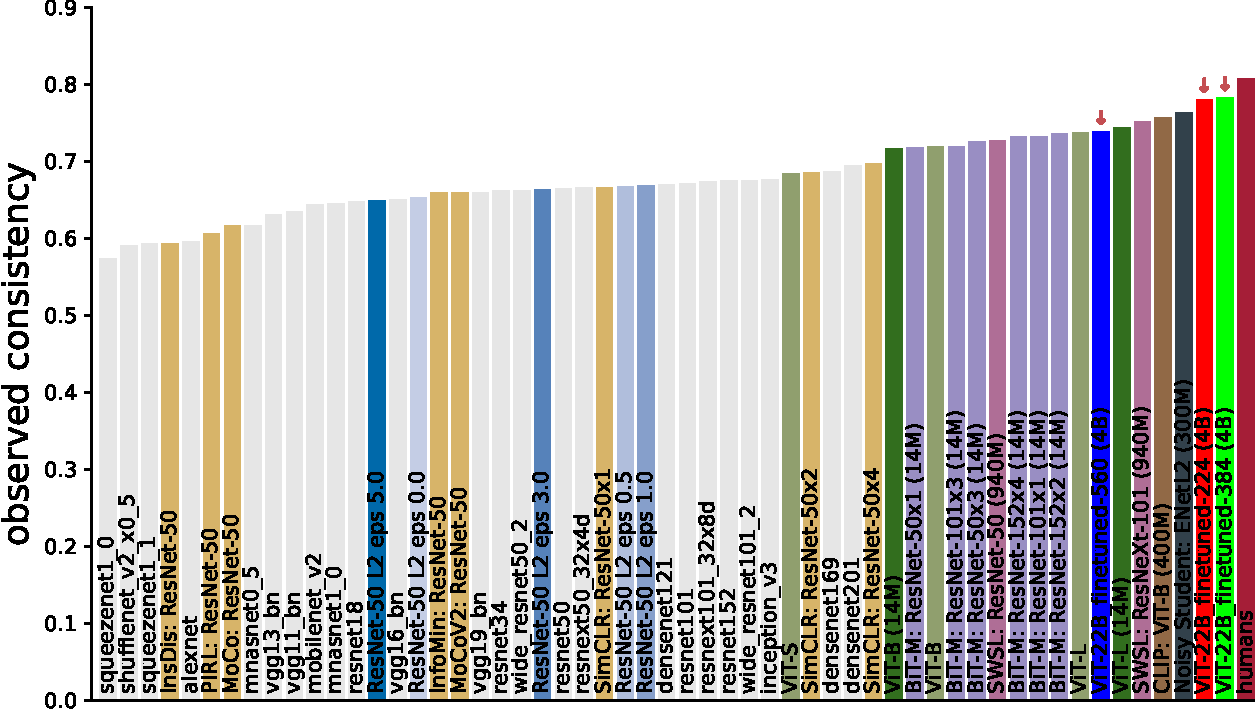
\includegraphics[height=1.6in]{figs/human-alignment/benchmark_observed-consistency.pdf}}
    \hspace{8pt}
    \subfigure[][Error consistency (higher = better).]{
        \label{fig:model_vs_human_benchmark_d}
        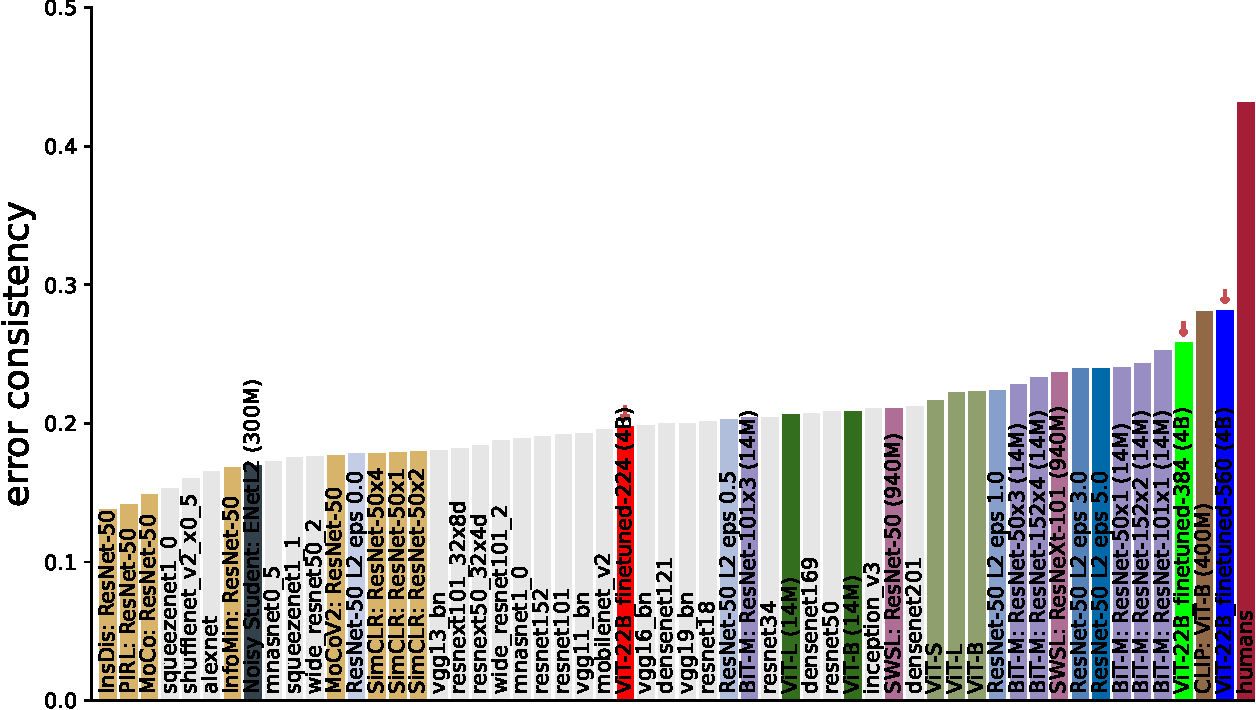
\includegraphics[height=1.6in]{figs/human-alignment/benchmark_error-consistency.pdf}}
    \caption[]{Model-vs-human~\citep{geirhos2021partial} benchmarking results for ViT-22B models fine-tuned on ImageNet with different resolutions (indicated by a red arrow). Results are aggregated over 17 challenging out-of-distribution (OOD) datasets from~\citep{geirhos2021partial}. OOD accuracy in \cref{fig:model_vs_human_benchmark_a} is simply the accuracy across those datasets; accuracy difference in \cref{fig:model_vs_human_benchmark_b} denotes the difference to human accuracies (either too low or too high is penalized); observed consistency in \cref{fig:model_vs_human_benchmark_c} shows unnormalized image-level consistency~\citep[see][for details]{geirhos2021partial} while \cref{fig:model_vs_human_benchmark_d} shows error consistency (normalizes observed consistency by the consistency expected purely by change). Error consistency is only above zero if models and humans systematically agree in terms of which images are easy/difficult (correct/incorrect classification). Overall, while the three ViT-22B variants trained with different resolutions vary in their performance, a ViT-22B variant leads the leaderboard in all four metrics. Comparison models include standard CNNs (grey), adversarially trained models (blue), self-supervised models (orange) as well as other models evaluated by \citet{geirhos2021partial}.}
    \label{fig:model_vs_human_benchmark}
\end{figure}

\section{Perceptual similarity}
\label{app:perceptual_similarity}
% Distances measured between images in the intermediate space of trained neural networks correspond to human assessments of similarity~\citep{zhang2018perceptual}. While~\citep{zhang2018perceptual} observe that the first generation of ImageNet classifiers such as AlexNet and VGG outperform low-level metrics significantly,
% In fact, models with low to medium ImageNet accuracy achieve the best perceptual scores.

\citet{kumar2022do} show a trade-off between the accuracy of latest ImageNet classifiers and their inherent ability to capture perceptual similarity. Here, we explore if large-scale classification on a more diverse training dataset than ImageNet can break the observed trade-off. To compare the perceptual similarity of \chonk with prior ImageNet-trained models, we make minor changes to adapt \chonk on low resolution $64 \times 64$ ImageNet. \chonk fine-tuned on ImageNet $64 \times 64$ achieves 84.2 accuracy on ImageNet $64 \times 64$ which is $16 \%$ better than the best models trained directly on ImageNet. As done in~\citep{zhang2018perceptual}, we assess the ability of \chonk to capture perceptual similarity using 48 intermediate representations. The perceptual score of \chonk (64.9) is much lower than all other models, indicating that models trained on large-scale classification also lie on the observed accuracy-perceptual similarity Pareto Frontier.

\begin{figure}[htbp]
    \centering
    \includegraphics[width=0.4\columnwidth]{figs/ps_vit22B.pdf}
    \caption{\chonk lies on the bottom-right of the accuracy-perceptual similarity tradeoff. It achieves the best validation accuracy on $64 \times 64$ ImageNet with the worst perceptual scores.}
    \label{fig:ps_vit22B}
\end{figure}

To make a fair comparison with the models in~\citep{kumar2022do}, we make minor changes to adapt ViT-22B on low resolution $64 \times 64$ ImageNet. Directly finetuneing ViT-22B on $64 \times 64$ images with the default patch-size of 14 leads to two undesirable consequences a) A low sequence length of 16 and b) Cropping of 8 pixels on the right borders. So, as proposed in~\citep{beyer2022flexivit}, we resize the trained embedding layer from the default patch-size of 14 to a patch-size of 8 that leads to a longer sequence length of 64. Then, we adapt standard finetuneing protocols.

We make three more observations: 1) Untrained ViT-22B gets a even lower Perceptual Score of 62.3, thus some amount of training is desirable 2) ViT-e lies in the same ballpark as ViT-22B with slightly lower accuracy and Perceptual Scores 3) ViT-22B with the newly proposed Mean Pool distance function~\citep{kumar2022do} can improve its Perceptual Score up to 66.2.


\section{Feature attribution analysis}
\label{app:feature_attribution}
To get a better understanding on how \chonk arrives at its predictions we make use of gradient-based feature attribution methods (a.k.a.\ saliency maps). 
\cref{fig:featureattribution} shows the result of applying Integrated Gradients~\citep[][IG]{sundararajan2017axiomatic} to three example datapoints before and after \chonk cooldown. We find that using a gray (0.5) baseline and 1024 steps yields qualitatively the best results. 
The images show a subtle difference in how the two model checkpoints process the example inputs, where more yellow indicates a higher sensitivity.
We can also clearly see the patches in which \chonk processes input images. This means that the model is less sensitive around the edges of each patch, and suggests a path for future work to improve the model to better deal with patch edges.

\begin{figure}[h]
    \centering
    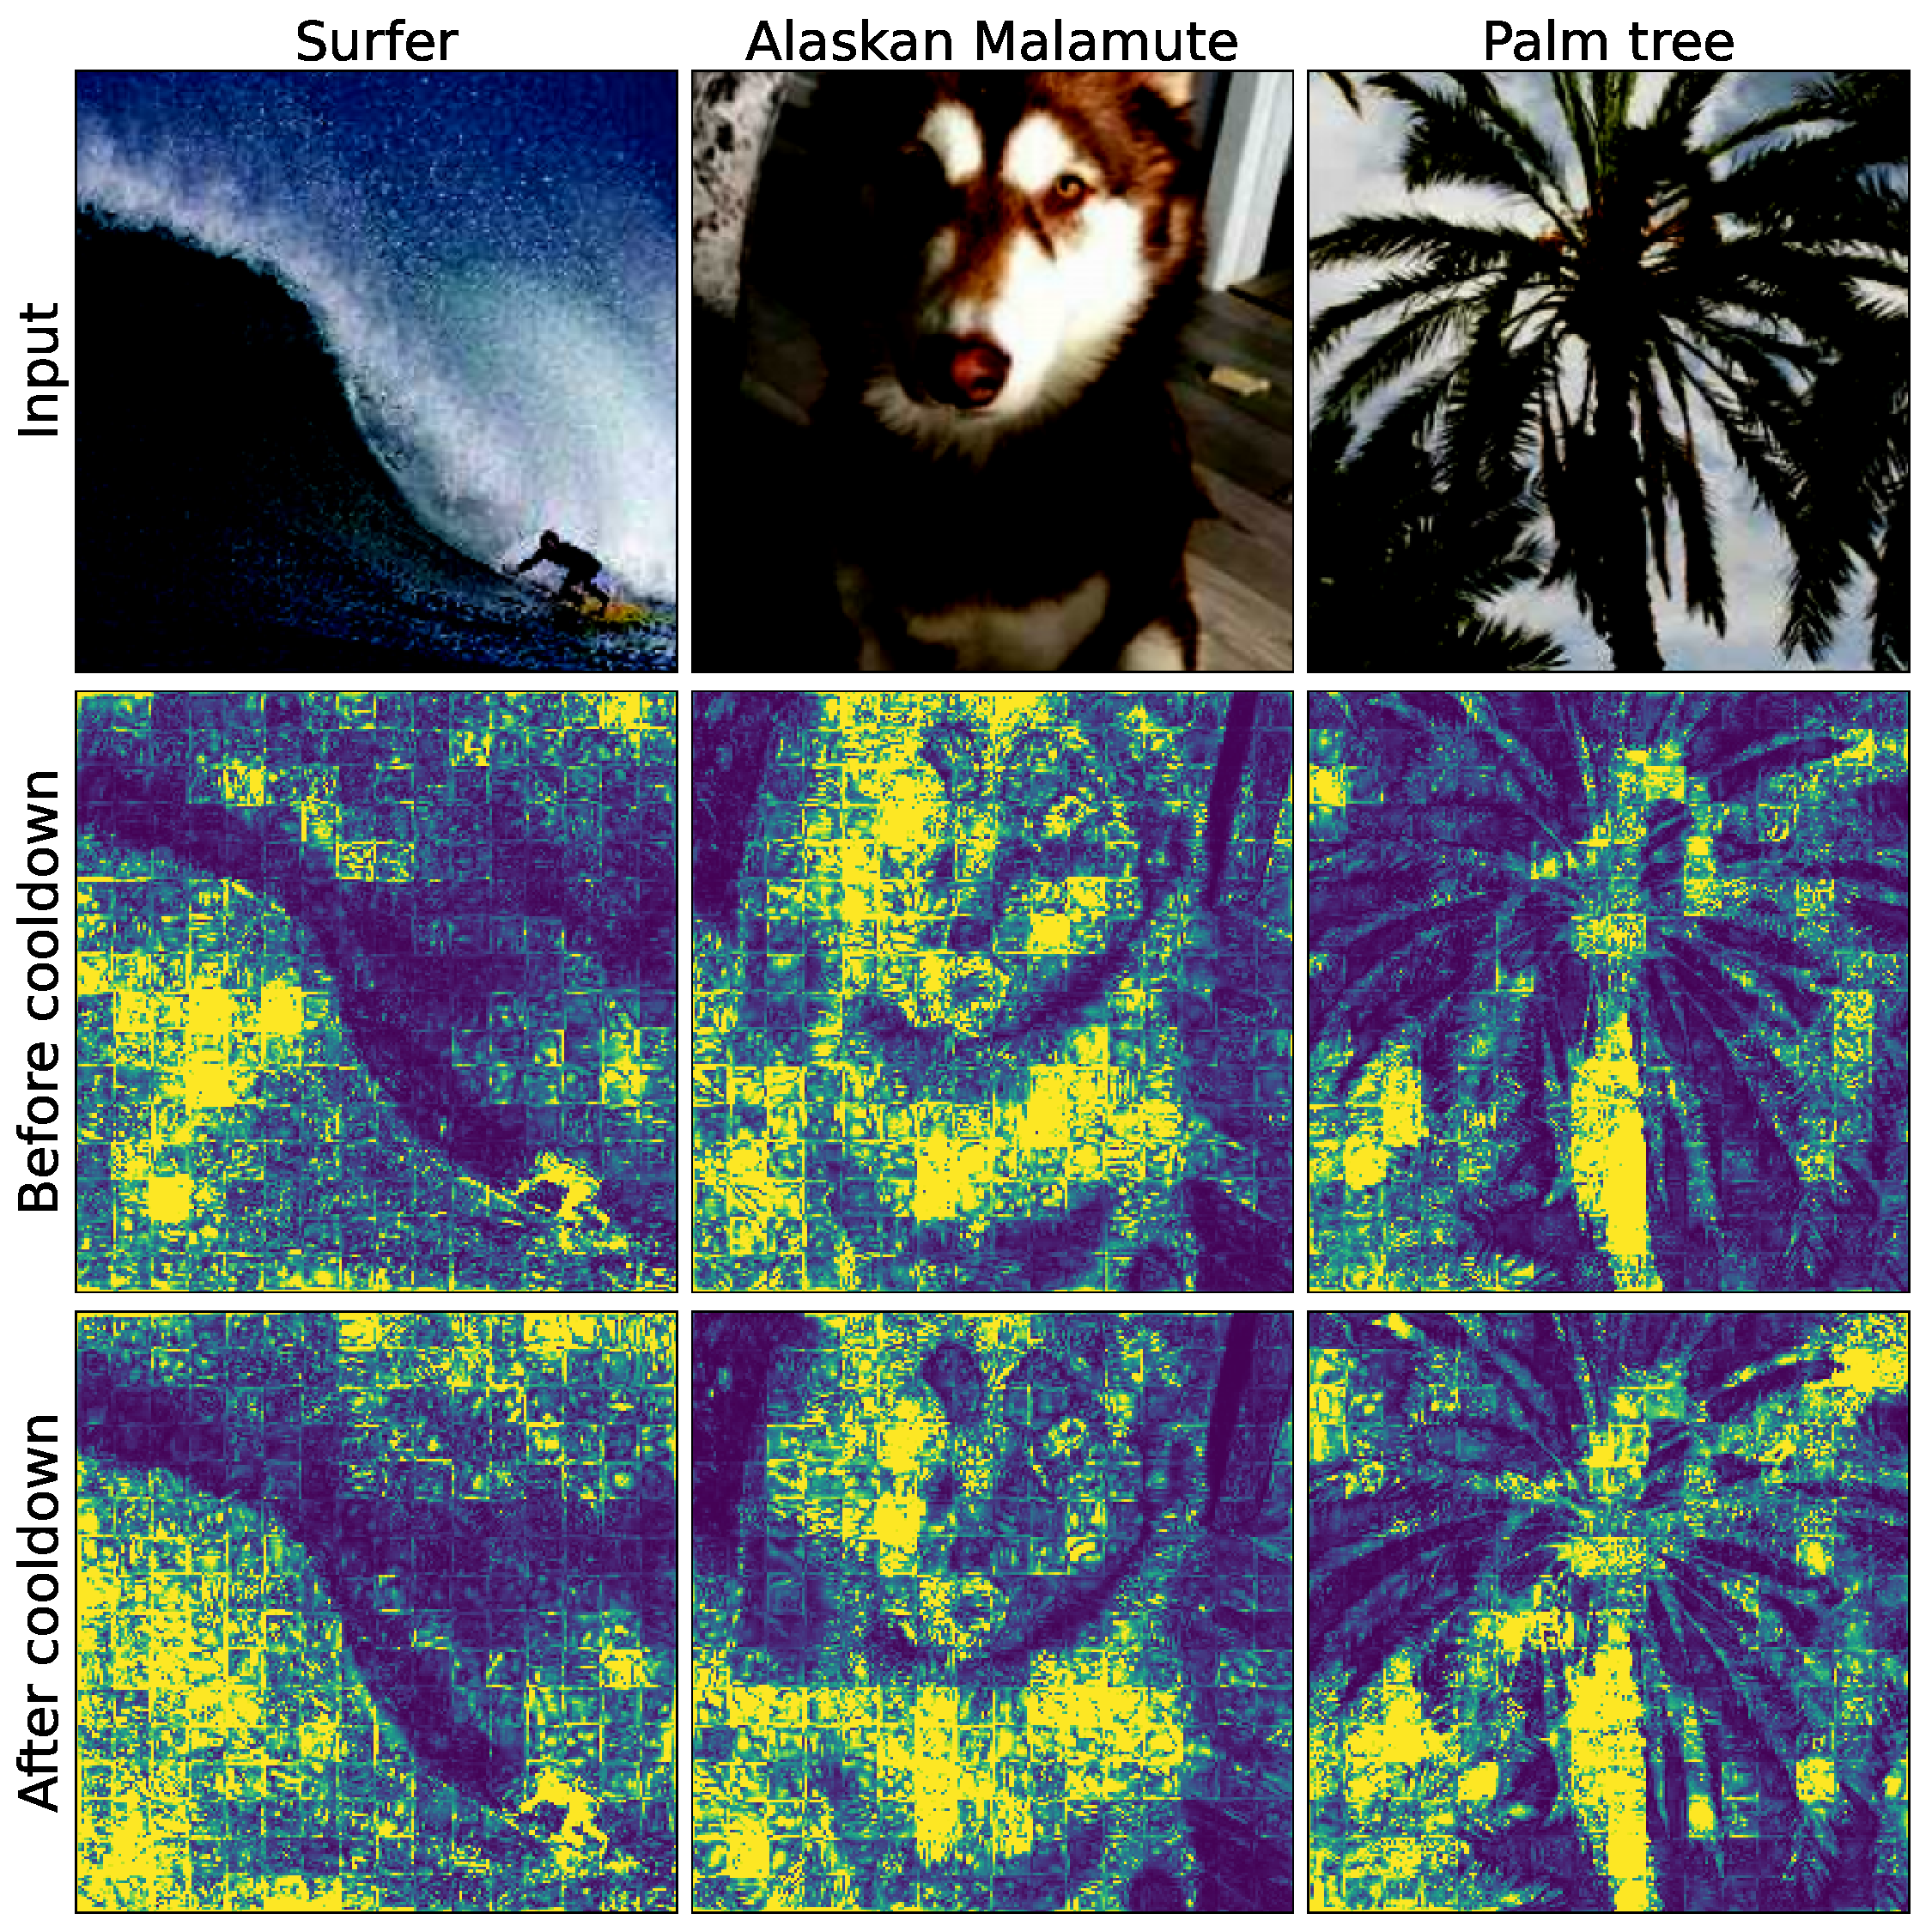
\includegraphics[width=0.5\textwidth]{figs/saliency/grads_ig}
    \caption{Saliency before and after model cooldown.}
    \label{fig:featureattribution}
\end{figure}